\documentclass[titlepage, a4paper]{article}
\usepackage[english]{babel}
\usepackage[utf8]{inputenc}
\usepackage{graphicx}
\usepackage{color}
\usepackage{mathtools}
\usepackage{float}
\usepackage[parfill]{parskip}
\usepackage[margin=10pt,font=small,labelfont=bf,labelsep=endash]{caption}
\usepackage{epstopdf}
\usepackage{listings}
\usepackage[table]{xcolor}
\usepackage{enumitem}
\epstopdfsetup{suffix=}
\DeclareGraphicsExtensions{.ps}
\DeclareGraphicsRule{.ps}{pdf}{.pdf}{`ps2pdf -dEPSCrop -dNOSAFER #1 \noexpand\OutputFile}


\definecolor{green}{rgb}{56,90,115}

\lstset{literate=%
    {å}{{\r{a}}}1
    {ä}{{\"a}}1
    {ö}{{\"o}}1
    {Å}{{\r{A}}}1
    {Ä}{{\"A}}1
    {Ö}{{\"O}}1
}

\newcommand{\todo}[1] {\textbf{\textcolor{red}{#1}}}

\usepackage{fancyhdr}
\fancyhead[L]{}
\pagestyle{fancy}
\rhead{Alexander Yngve \\ Pål Kastman}
\chead{TDTS08}
\thispagestyle{empty}

\begin{document}

{\ }\vspace{45mm}

\begin{center}
  \Huge \textbf{TDTS08: Lab Report}
\end{center}
\begin{center}
  \Large Lab 2: Instruction Pipelining
\end{center}

\vspace{250pt}

\begin{center}
  \begin{tabular}{|*{3}{p{40mm}|}}
    \hline
    \textbf{Name} & \textbf{PIN} & \textbf{Email} \\ \hline
           {Alexander Yngve} & {930320-6651} & {aleyn573@student.liu.se} \\ \hline
           {Pål Kastman} & {851212-7575} & {palka285@student.liu.se} \\ \hline
  \end{tabular}
\end{center}
\newpage

\tableofcontents
\thispagestyle{empty}
\newpage

\section{Introduction}
The purpose of this lab is to learn how instruction pipelining works and how branch prediction affects the performance of the pipeline.

\section{Pipeline basics I}

\begin{figure}[H]
  \centering
  \begin{tabular}{|c|c|c|c|c|c|}
    \hline
    \cellcolor{blue!25}{IF} &
    \cellcolor{orange!25}{DA} &
    \cellcolor{blue!25}{CO} &
    \cellcolor{orange!25}{FO} &
    \cellcolor{blue!25}{EX} &
    \cellcolor{orange!25}{WB} \\ \hline
  \end{tabular}
  \caption{Six stage pipeline.}
  \label{fig:pipeline}
\end{figure}


\begin{description}[leftmargin=!,labelwidth=\widthof{\bfseries WB}]
\item[LB instruction]
\item[IF] fetch instruction in memory.
\item[DA] activate different parts in the cpu depending on the instruction.
\item[CO] calculate the address in the memory where the operand is stored. 
\item[FO] fetch operand from memory.
\item[EX] not used.
\item[WB] write operand to register.
\end{description}
~\newline

\begin{description}[leftmargin=!,labelwidth=\widthof{\bfseries WB}]
\item[ADD instruction]
\item[IF] fetch instruction in memory.
\item[DA] activate different parts in the cpu depending on the instruction.
\item[CO] calculate the address in the memory where the operand is stored. 
\item[FO] fetch operand from memory.
\item[EX] compute addition.
\item[WB] write result to register.
\end{description}
~\newline

The main difference for the two instruction is that LB doesn't need to use the instruction execute (EX) state, since its only loading data from the memory.

\section{Pipeline basics II}
When we have a short pipeline we get less time penalty due to that its only one step that needs redoing and therefore its detected earlier. \\

\begin{figure}[H]
  \centering
  \begin{tabular}{|c|c|c|c|c|c|}
    \hline
        {} & {1} & {2} & {3} & {4} & {5} \\ \hline
        {1} & \cellcolor{blue!25}{IF} & \cellcolor{orange!25}{EX} & {} & {} & {} \\ \hline
        {2} & {} & \cellcolor{blue!25}{IF} & \cellcolor{orange!25}{EX} & {} & {} \\ \hline
        {3} & {} & {} & \cellcolor{blue!25}{IF} & \cellcolor{orange!25}{EX} & {} \\ \hline
        {4} & {} & {} & {} & \cellcolor{blue!25}{IF} & \cellcolor{orange!25}{EX} \\ \hline
  \end{tabular}
  \caption{Ideal pipeline operation.}
  \label{fig:ideal_pipe_op}
\end{figure}

\begin{figure}[H]
  \centering
  \begin{tabular}{|c|c|c|c|c|c|c|}
    \hline
        {} & {1} & {2} & {3} & {4} & {5} & {6} \\ \hline
        {1} & \cellcolor{blue!25}{IF} & \cellcolor{orange!25}{EX} & {} & {} & {} & {} \\ \hline
        {2} & {} & \cellcolor{blue!25}{IF} & \cellcolor{orange!25}{EX} & {} & {} & {} \\ \hline
        {25} & {} & {} & \cellcolor{blue!25}{IF} & {} & {} & {} \\ \hline
        {4} & {} & {} & {} & \cellcolor{blue!25}{IF} & \cellcolor{orange!25}{EX} & {} \\ \hline
        {5} & {} & {} & {} & {} & \cellcolor{blue!25}{IF} & \cellcolor{orange!25}{EX} \\ \hline
  \end{tabular}
  \caption{Pipeline operation during conditional jump.}
  \label{fig:condjmp_pipe_op}
\end{figure}

\section{Branch prediction}
Here we analyze how the different branch prediction algorithms perform.

\subsection{Desciption}
For each predictor a benchmark was run according to the following command

$$\text{sim-outorder -bpred \textit{predictor} $\mathtt{\sim}$/TDTS08/bin/go.ss 3 8}$$

The different algorithms works as following:

\begin{description}[leftmargin=!,labelwidth=\widthof{\bfseries NOTTAKEN}]

\item[TAKEN] Assumes the jump is always taken.
\item[BIMOD] Address of the branch instruction is used as a key into an associative memory where a two bit saturating counter is stored, when branch is taken the counter is incremented and vice versa. The branch will look on the msb to determine direction.
\item[2LEV] Current branch instruction has a set of saturating counters which is choosen depending on the history of the branch, this history is stored in a shift register.
\item[COMB] Combination of bimod and 2lev.
\item[PERFECT] This one cheats and always chooses the correct branch.
\item[NOTTAKEN] Assumes the jump is never taken.
\end{description}
~\newline

\subsection{Result}
The performance result can be seen in figure \ref{fig:performance} below.

\begin{figure}[H]
	\centering
	\scalebox{0.342}{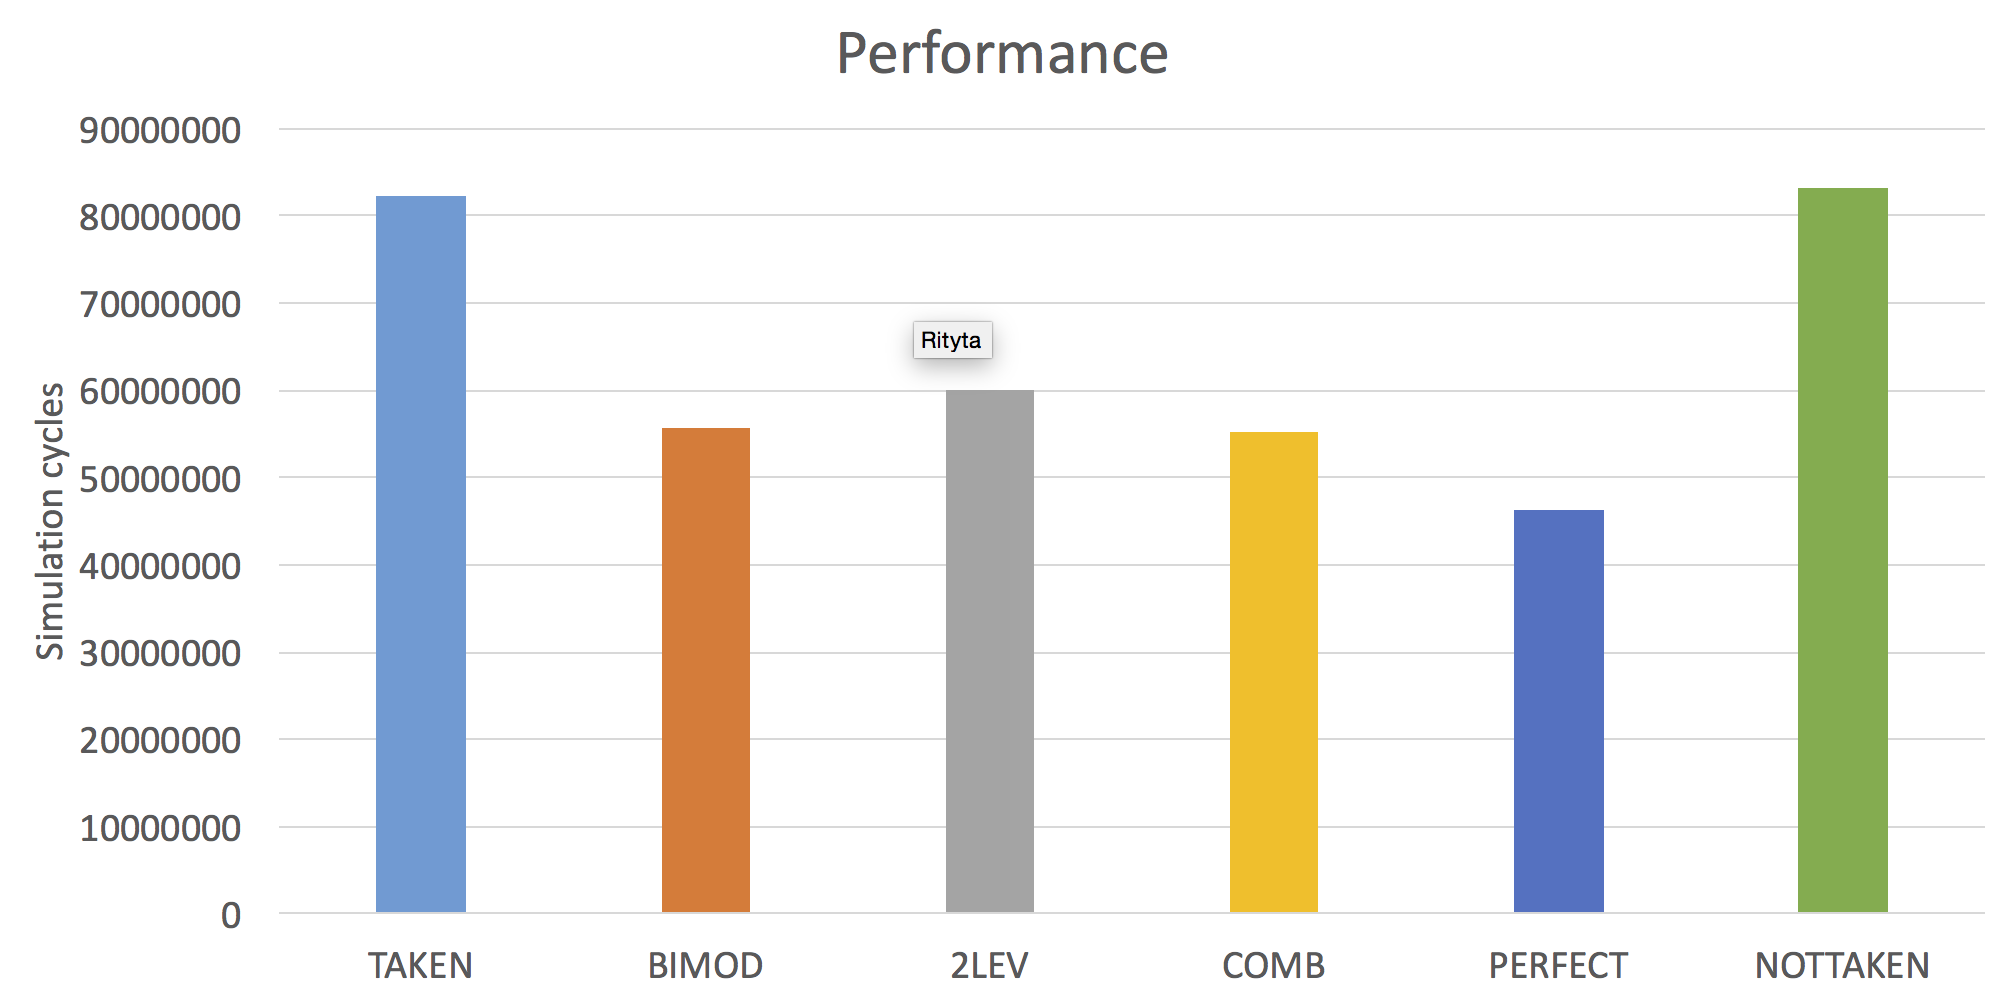
\includegraphics{img/performance-cycles.png}}
	\caption{Performance of the different branch prediction algorithms}
	\label{fig:performance}
\end{figure}

In figure \ref{fig:performance} we can see that the \textit{not taken} algorithm performs worst. If we look at how the algorithms perform according to each other, and we originate from the \textit{not taken} algorithm since it performs the worst, we then get a result according to figure \ref{fig:comparative-evaluation}. The results in figure \ref{fig:comparative-evaluation} are based on the direction rate metric (bpred\_dir\_rate).

\begin{figure}[H]
	\centering
	\scalebox{0.342}{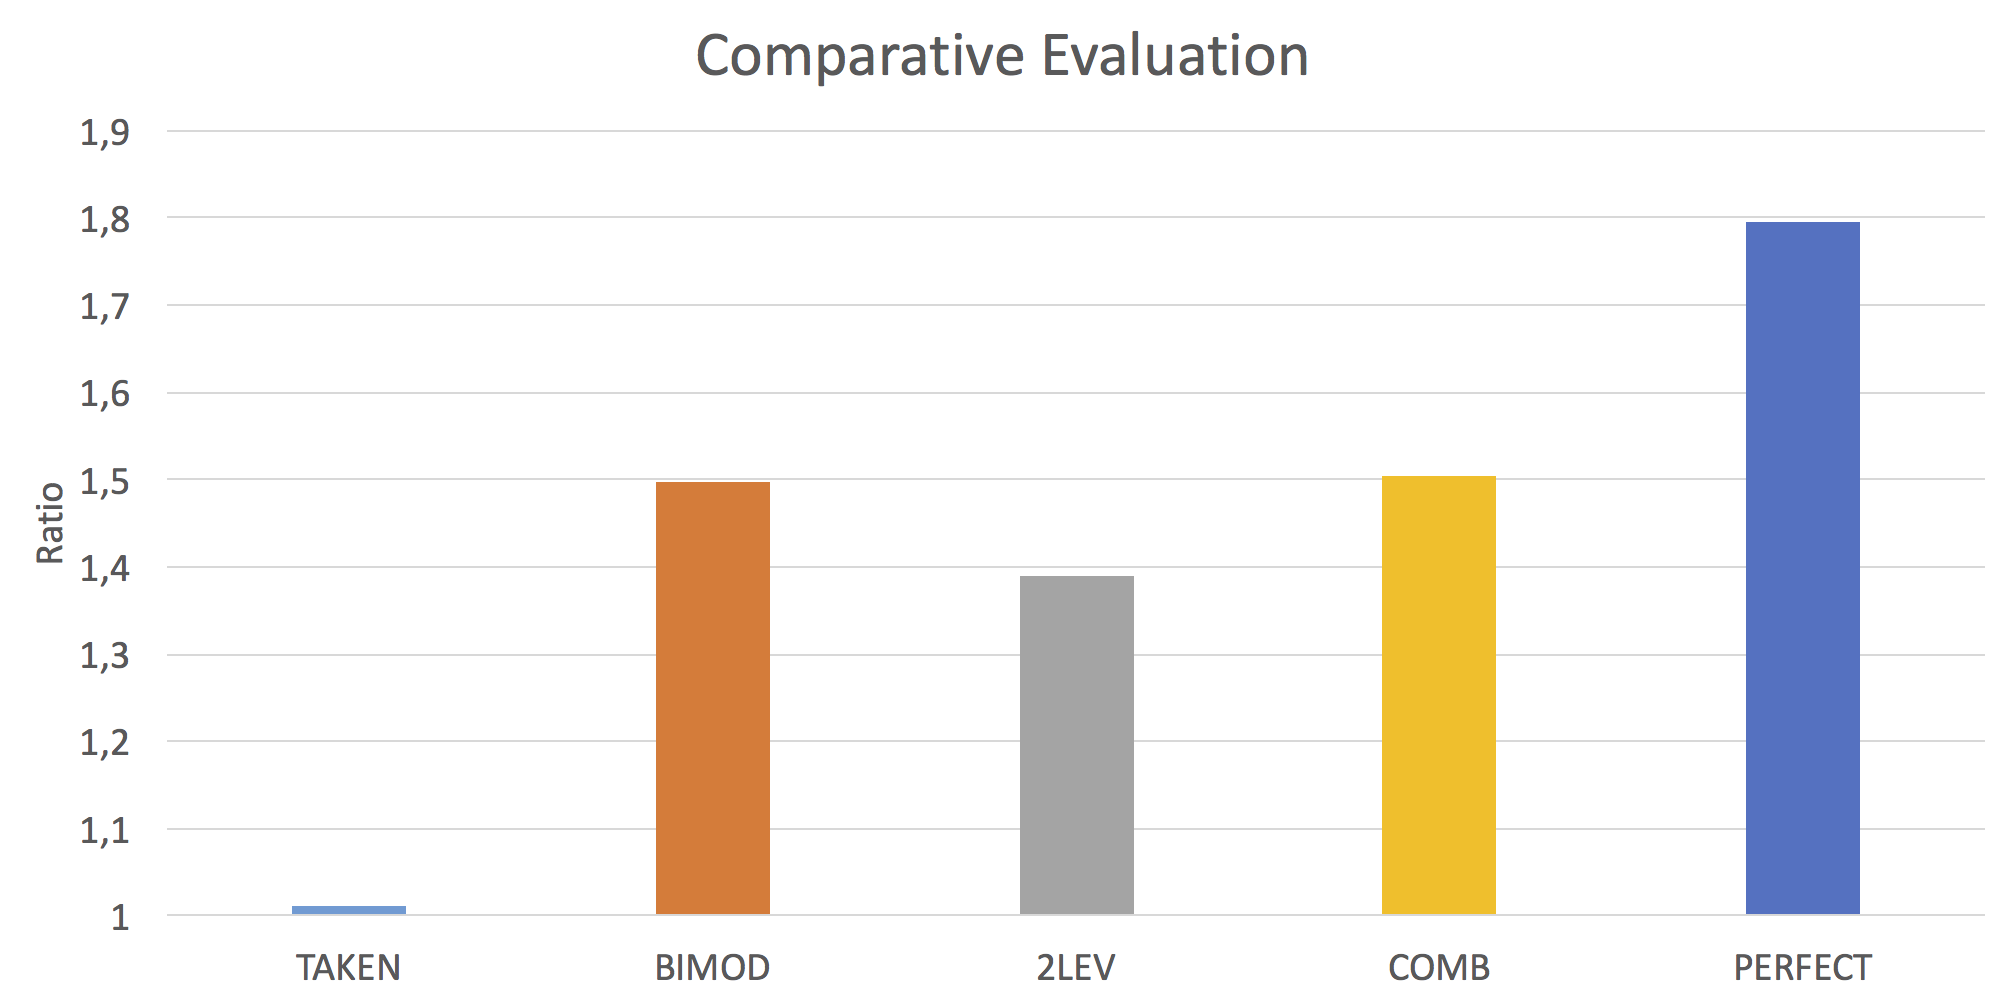
\includegraphics{img/comparative-evaluation.png}}
	\caption{Performance of the alogorithm according to the not taken algorithm who performed worst.}
	\label{fig:comparative-evaluation}
\end{figure}

\end{document}
